\documentclass[12pt]{report}
\usepackage{listings}
\usepackage{color}
\usepackage{graphicx}
\usepackage[english]{babel}
\usepackage{graphicx}

\begin{document}



\begin{figure}[!bh]
	\begin{center}
		\title{This is the examination of Essential skills: \LaTeX}
		\author{Florian Ecard, 10874763, Master SNE, UvA} 
		\date{2014\\}
	\maketitle 
		
\includegraphics{uva.jpeg}
		\label{sec:uva}
	\end{center}
\end{figure}


\newpage

	\tableofcontents

\newpage
\chapter{Introduction}
	\section{General aim}
		\subsection{aim of this report}
			\begin{itemize}
				\item In this exam, the following will be investigated:
				\begin{enumerate}
					\item Being able to create a short report
					\item Containing different parameters such as an image, a table etc. 
				\end{enumerate}
				\item If you proove your skills then you should be able to pass this exam.
			\end{itemize}
		\subsection{What is expected from us}
		Having two research projects to do, it is important to be able to present a report properly. Latex is very useful and easy to use for these purposes and this is why we learn it and that it is part of our essential skills. 
			
			
			
\chapter{Contribution}
	\section{Table, Maths and picture}
		\subsection{Table}
		
		\begin{table}[!h] \label{sec:table}
		\begin{center}
			\begin{tabular}{|l||c|r} 
				Is this going to be corrected? & Nothing's less sure..\\
				do you hope so? & Hell yeah!\\
			\end{tabular}
			\caption{Is my exam going to be corrected?}
		\end{center}
		\end{table}
		
		\begin{enumerate}
			\item Does this table looks nice?
			\item Or this table doesn't?
			\item I don't really know what to write here ... 
		\end{enumerate}
		
		
		\subsection{Mathematics}
			\begin{itemize}
			 	\large \item \(x= \frac{x+z/2}{y ^{2}+1}\)		(1) \label{sec:math} 
			 	\item \(y= \frac{y+n/2}{x ^{2}+1}\) 
			\end{itemize}
			
		
		\newpage
		\subsection{Figure}
			\begin{figure}[h!] \label{sec:image}
				\begin{center}
					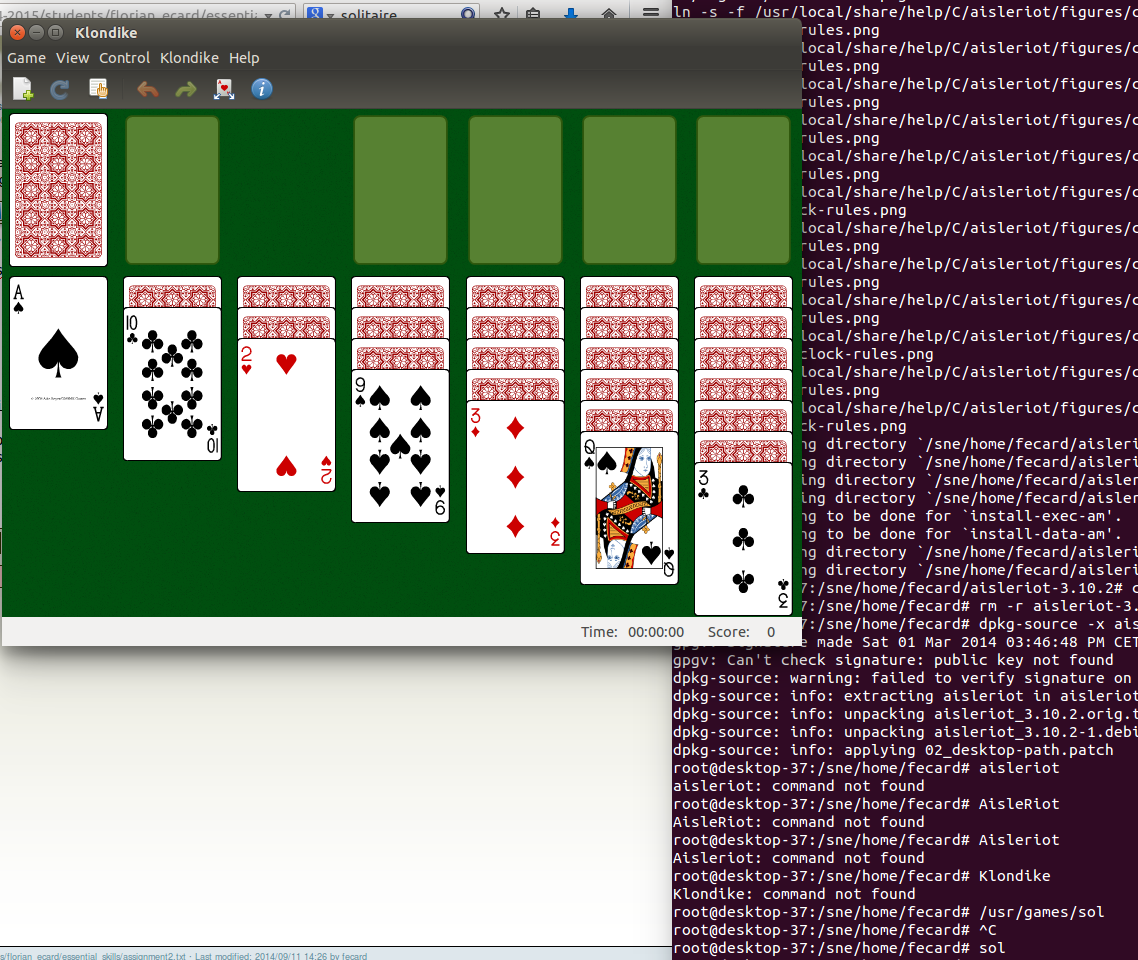
\includegraphics[scale=0.2]{sol.png}
					\caption{Image of the downloaded game for the build tools Assignment}
				\end{center}
			\end{figure}
			
			
\chapter{Conclusions}
	\section{What was this?}
	We covered how to create a nice document with \LaTeX
		\subsection{What did we do?}
			\begin{itemize}
				\item This was a nice exam
				\item The following topics were covered:
				\begin{enumerate}
					\item Provide the correct syntax of a good report 
					\item Show tables 
					\item Show images 
					\item Show mathematics
					\item Give a table of contents, and bibliography
				\end{enumerate}
			\end{itemize}




\begin{thebibliography}{9}
\bibitem{logo}
wget http://goo.gl/QMRWRs -O uva.jpeg \textbf{Which is in page } \pageref{sec:uva}

\bibitem{table}
The table is in page \pageref{sec:table} in section \ref{sec:table}

\bibitem{mathematics}
The maths are in page \pageref{sec:math} in section \ref{sec:math}

\bibitem{image}
The image is in page \pageref{sec:image} in section \ref{sec:image}
\end{thebibliography}

\end{document}